\section{Так квинтовый или квартовый? Квинто-квартовый круг}
\label{ch:harmony:kvinto-kvarto-round}

На самом деле полное название этого полезного помошника, которго легко сделать из бумаги: <<квинто-квартовый круг мажорных и минорных тональностей>>. Выглядит он странно: см. рисунок \ref{TODO}. И хотелось бы не только научиться им пользоваться, но и понять почему он именно такой.

TODO рисунок

Круг может помочь, если вы хотите:
\begin{itemize}
    \item Подобрать <<сочетающиеся>> аккорды для аккомпанемента песен.
    
    \item Определить, какие ноты входят в ту или иную мажорную или минорную тональность.
    
    \item Сменить <<тональность>> аккомпанемента песни. Человеческим языком: \emph{каждую} ноту исходной тональности нужно повысить или понизить на заданное количество полутонов. Зачем? Чтобы было удобнее петь. При этом интервальная структура (т.е. характер, например, веселый или грустный) музыки не изменится, а произведение <<в целом>> будет звучать ниже или выше, <<подстраиваясь>> таким образом под голос исполнителя.    

    \item Решить <<академические>> задачки, например, определить тональность произведения по нотам или определить параллельную тональность.
    
    \item И много чего ещё\ldots
\end{itemize}

Мы не будем сейчас учиться как решать эти задачки, мы начнем разбираться с устройством круга. А в процессе станет понятно не только, как решать эти задачки, но и многое другое.

Глядя на рисунок \ref{fig:harmony:interval:octave-kon-dis} можно увидеть, что для отдельно взятого звука в пределах октавы существует лишь \emph{два} звука, образующий с исходным звуком совершенный консонанс. Относительно исходного эти звуки находятся на расстоянии в 5 (кварта) и 7 (квинта) полутонов. Оказывается, что можно переупорядочить ноты так, чтобы совершенные консонансы стали соседями исходного звука: один справа, другой слева!

Начнём, например с ноты ДО, и отступая по семь полутонов по часовой стрелке:
\[
    C\rightarrow 
    G\rightarrow 
    D\rightarrow 
    A\rightarrow 
    E\rightarrow 
    B\rightarrow 
    {F\sharp}\rightarrow
    {C\sharp}\rightarrow
    {G\sharp}\rightarrow
    {D\sharp}\rightarrow
    {A\sharp}\rightarrow
    F\rightarrow 
    C
\]
замкнем круг и получим результат, представленный на рисунке \ref{fig:harmony:kvinto-kvarto:kons-rearrange}.

\begin{figure}[!ht]
    \centering
    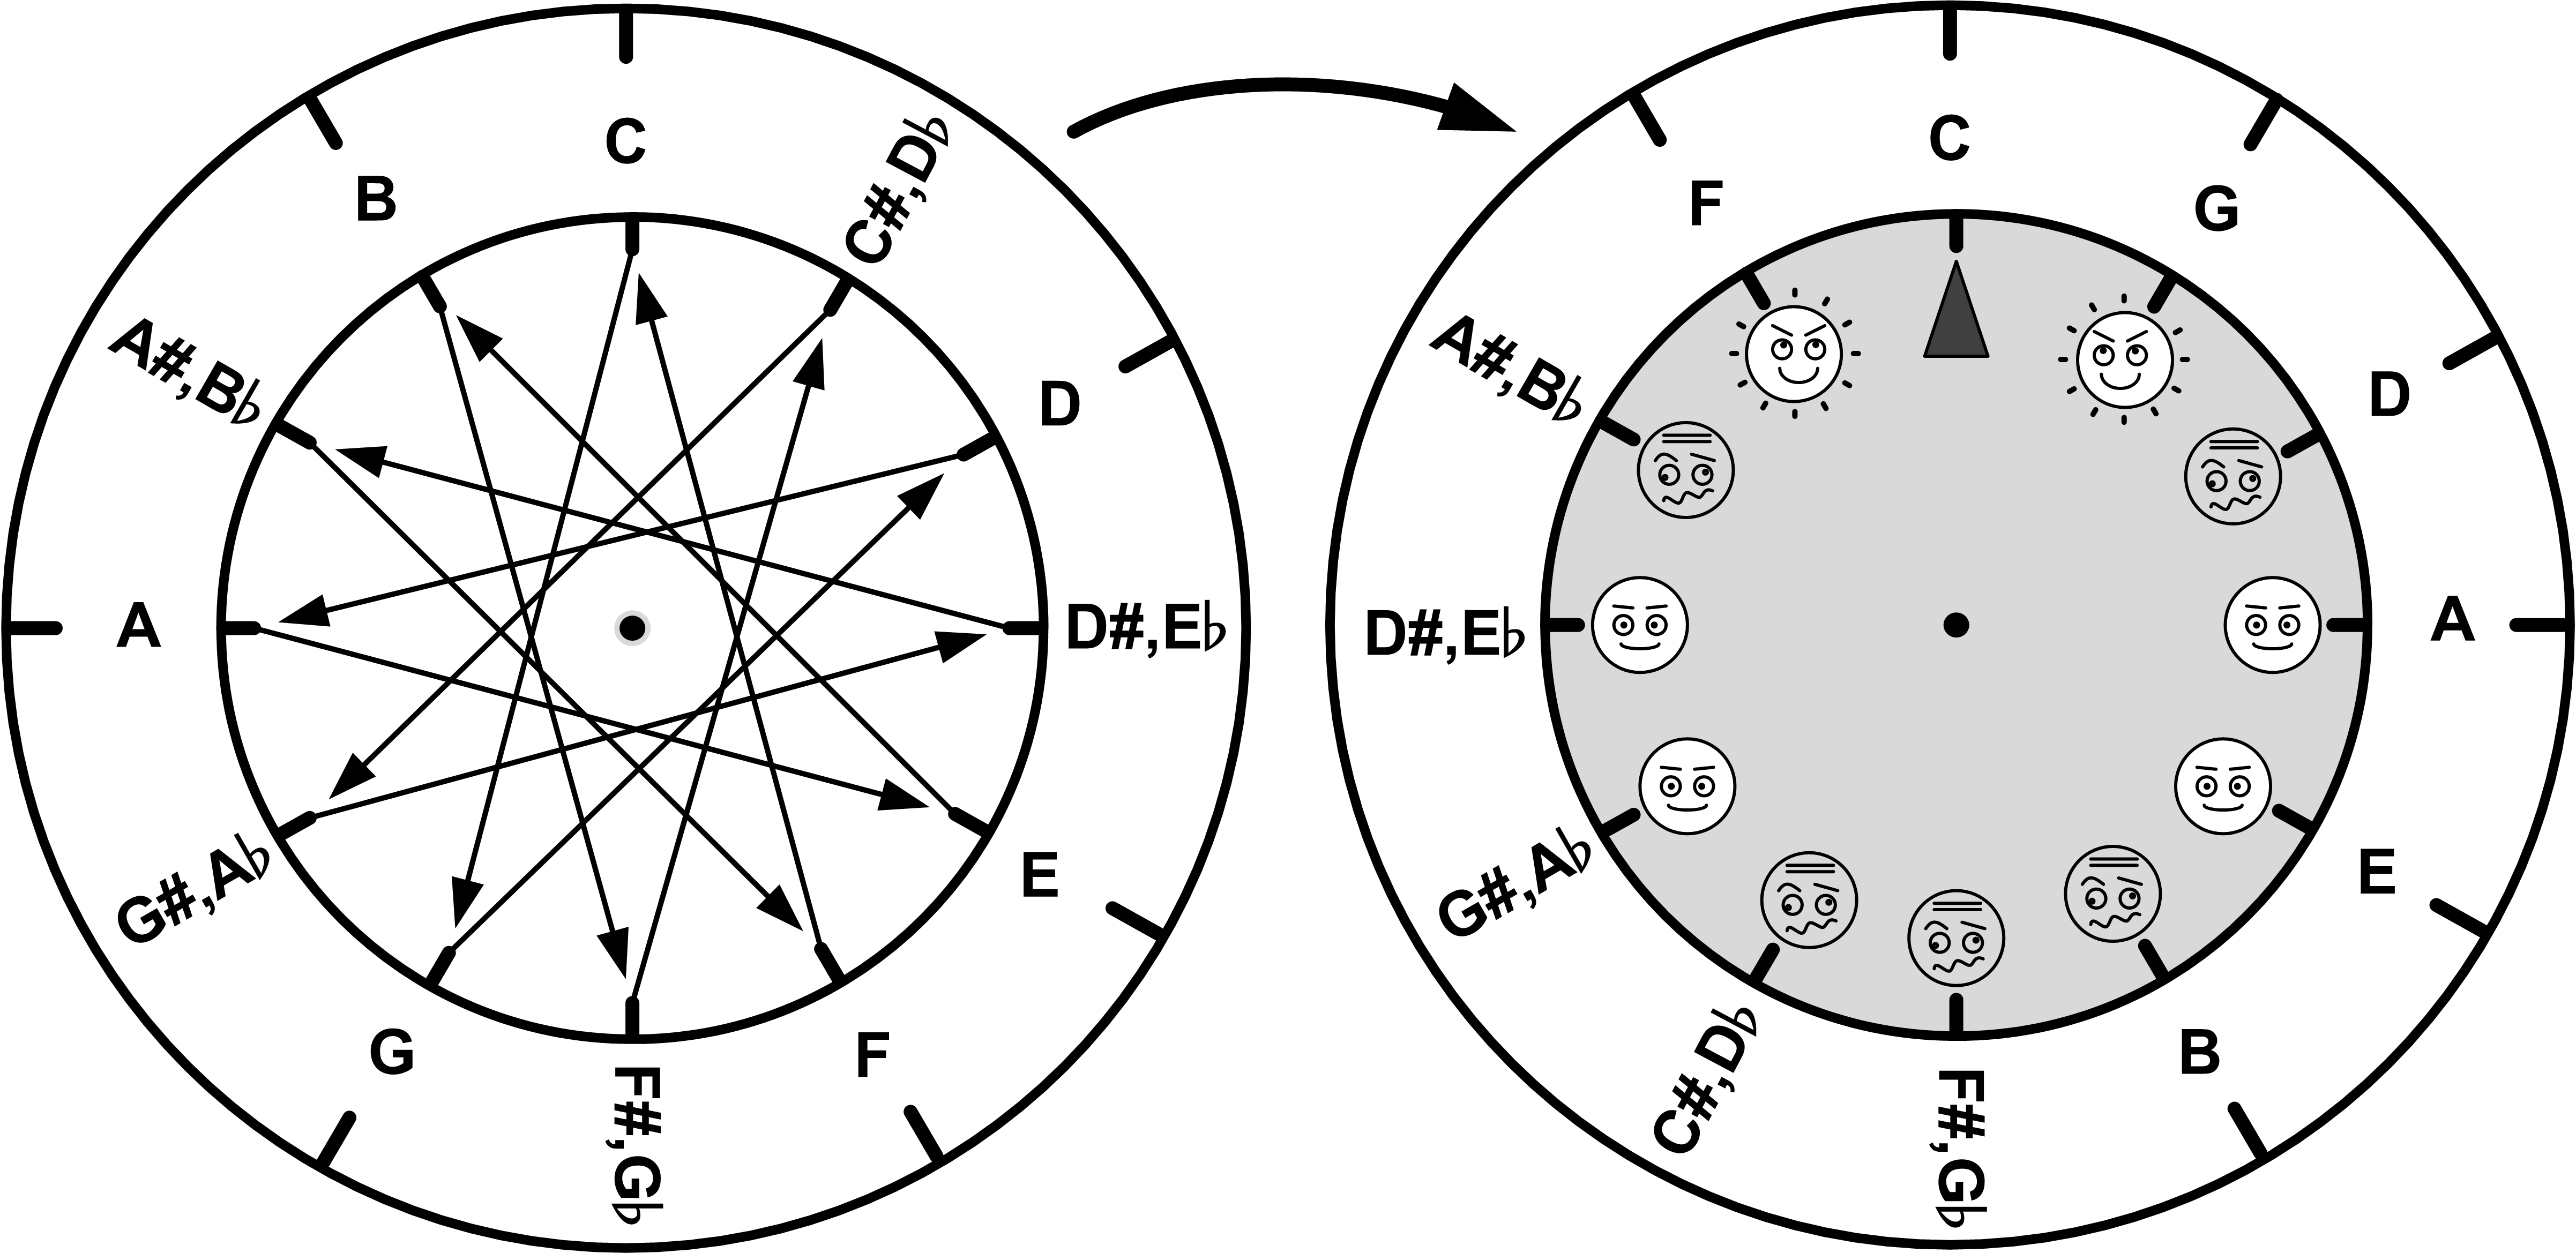
\includegraphics[scale=0.7]{fig/kvinto-kvarto/kons-rearrange} 
    \caption{Консонансы по соседству}\label{fig:harmony:kvinto-kvarto:kons-rearrange}
\end{figure} 

Теперь достаточно ткнуть в любую ноту на получившемся круге и узнать её совершенные консонансы: соседом против часовой стрелки будет совершенный консонанс на расстоянии 5 полутонов (чистая кварта), а по часовой --- консонанс на расстоянии 7 полутонов (чистая квинта). Например, возмьем ноту ЛЯ(A) и сразу определяем консонансы: РЕ(D) --- кварта от ЛЯ и МИ(E) --- квинта.

Обратите внимание на то, что среди переупорядоченных нот явно выделились две цепочки: цепочка нот без диезов и бемолей и цепочка нот со знаками альтерации. Конечно, это не случайность: ноты без диезов и бемолей --- это названия ступеней мажорного лада (а точнее --- тональность ДО-мажор). И само-собой, мажорный лад в своё время был сформирован с учетом расположения совершенных консонансов и вполне возможно, автор при этом глядел на полученный нами круг.

Итак, ноты тональности ДО-мажор выстроились в одну цепочку. При этом тоника --- ДО, идет в этой последовательности второй, если считать по часовой стрелке.

Таким образом упростилась задача определения нот для \emph{любой} мажорной тональности: 
\begin{enumerate}
    \item нужно отметить тонику на круге и отступить от нее на один сектор против часовой стрелки;
    \item включая полученную ноту, двигаясь по часовой стрелке, отсчитать семь нот тональности.
\end{enumerate}

Например, требуется определить ноты тональности РЕ-мажор (см. рисунок \ref{fig:harmony:kvinto-kvarto:d-maj}). Отступаем от $D$ против часовой стрелки, а затем по часовой собираем 7 нот:
\[
    G\rightarrow 
    D\rightarrow 
    A\rightarrow 
    E\rightarrow 
    B\rightarrow 
    {F\sharp}\rightarrow
    {C\sharp}
\]

\begin{figure}[!ht]
    \centering
    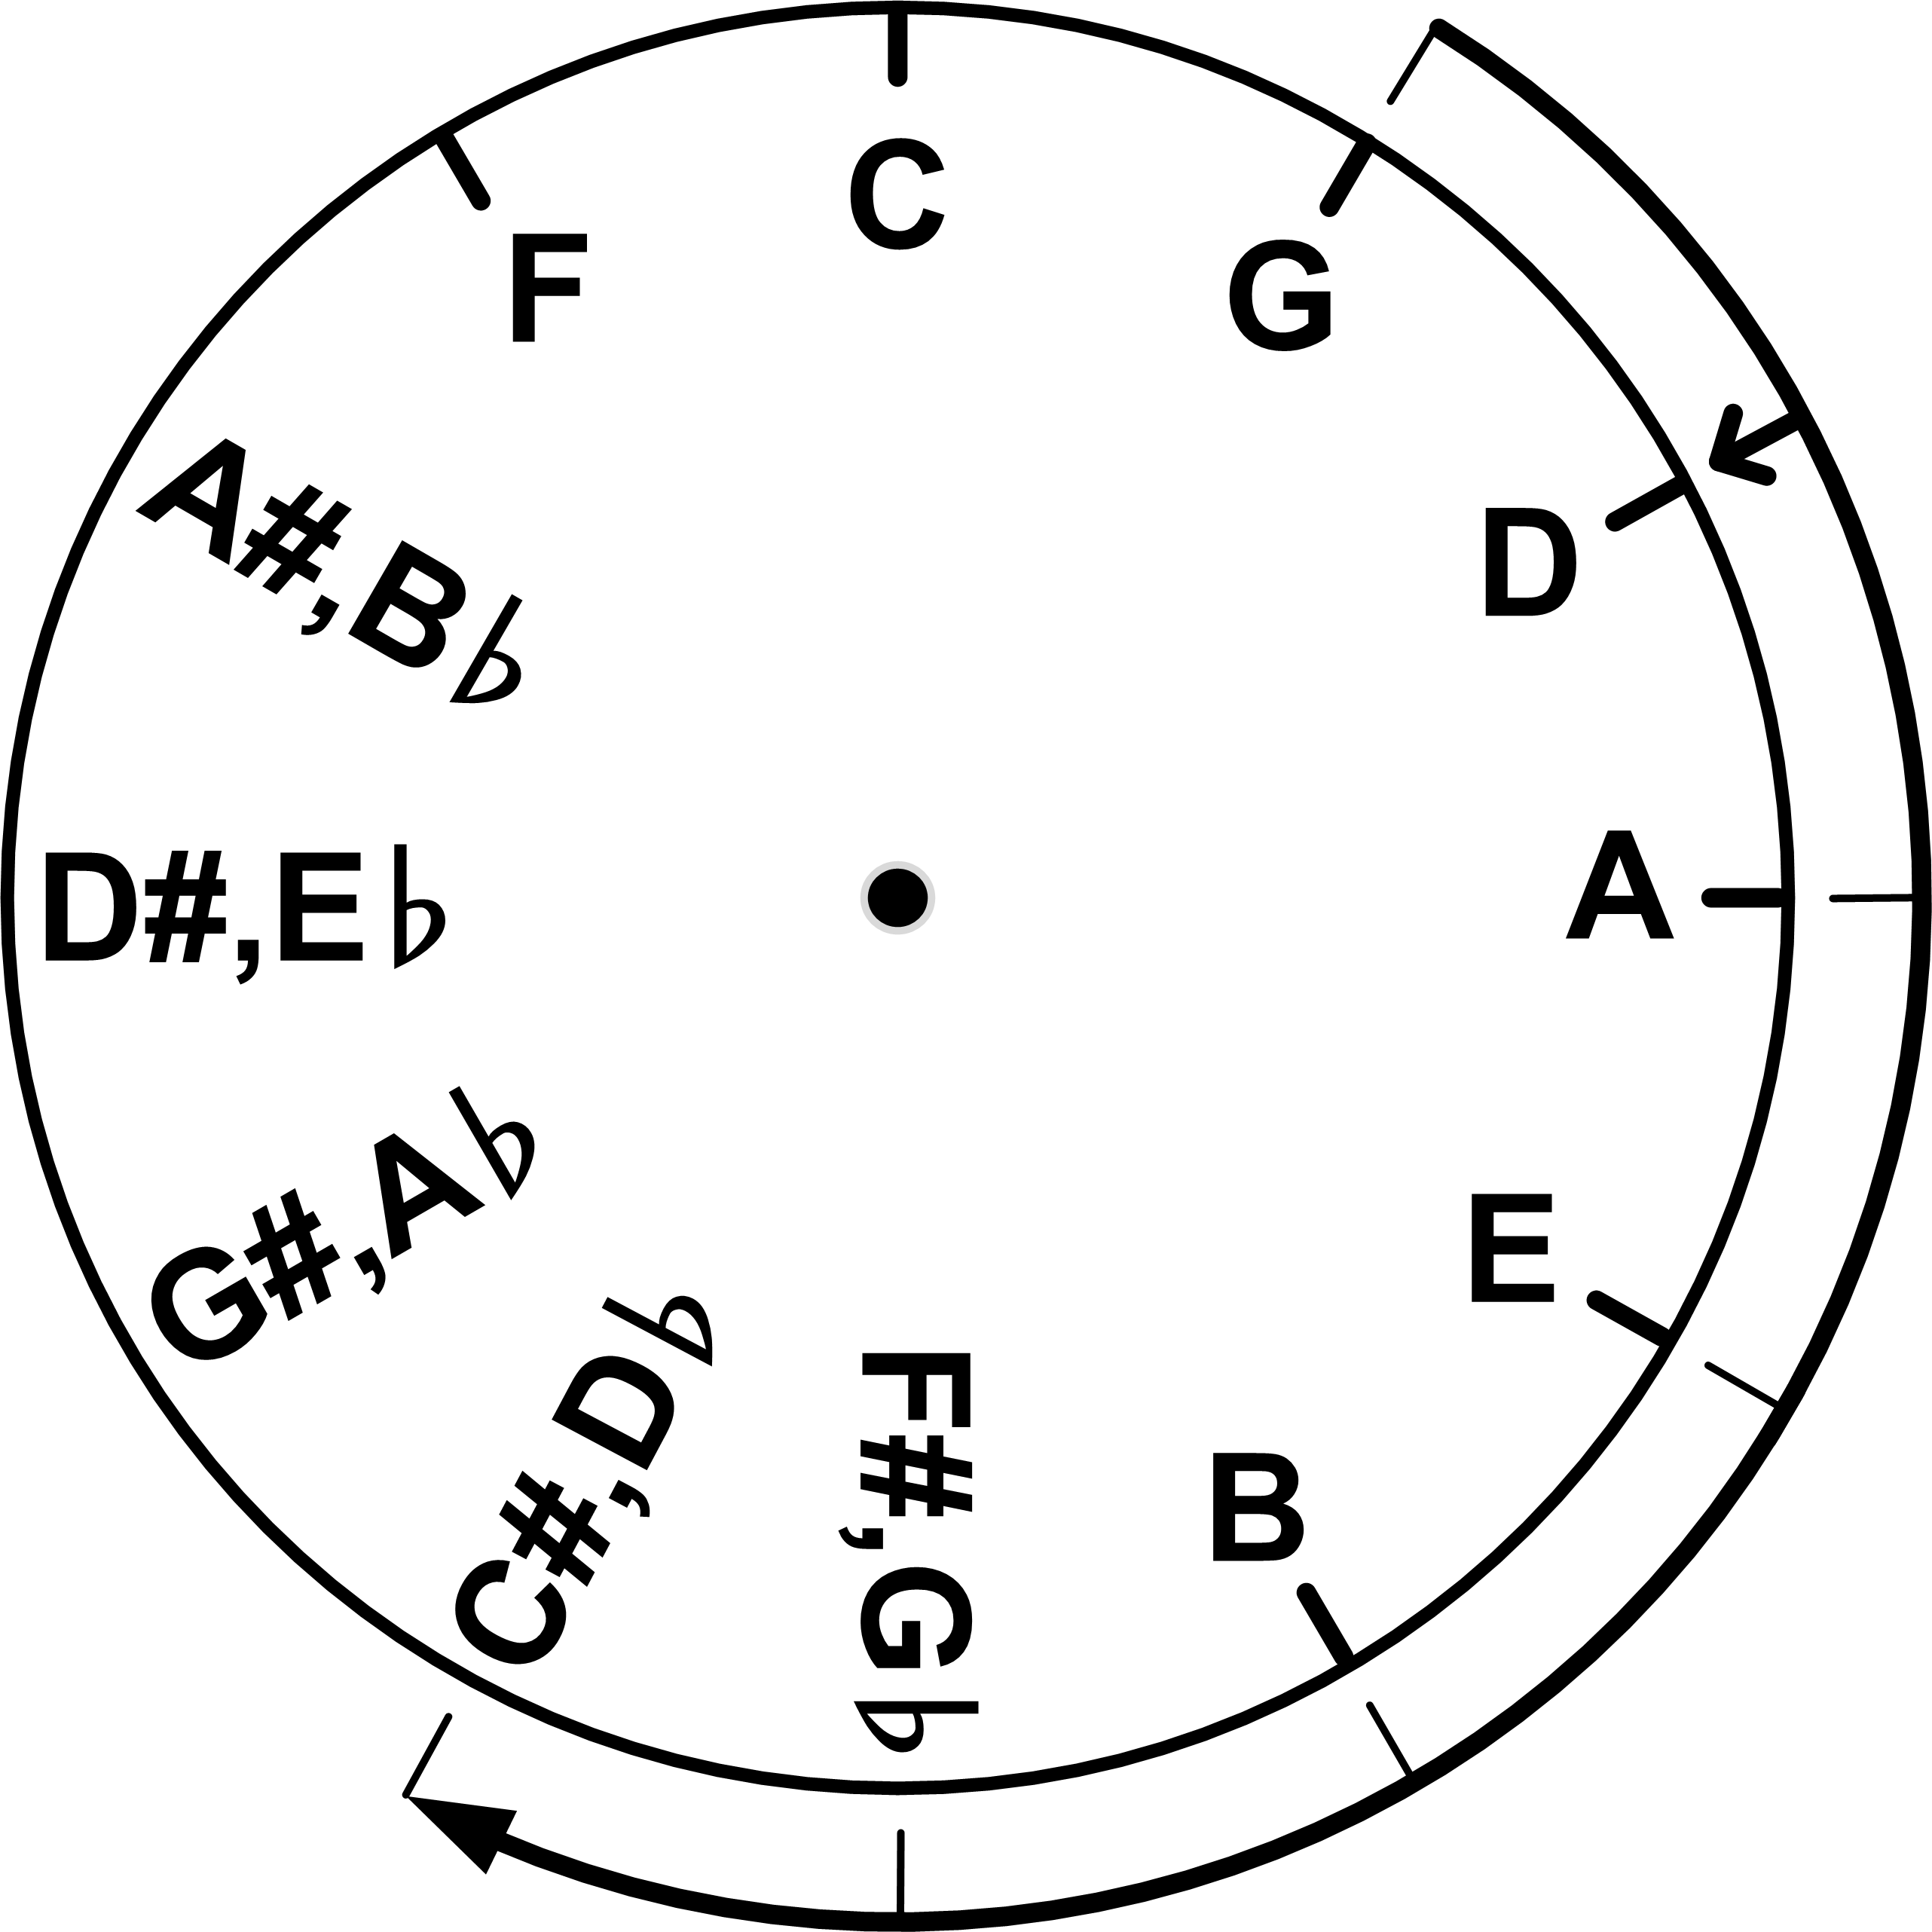
\includegraphics[scale=0.5]{fig/kvinto-kvarto/kvinto-kvarto-d-maj} 
    \caption{Ноты тональности D-maj}\label{fig:harmony:kvinto-kvarto:d-maj}
\end{figure}

Естественно, что ноты по высоте пока не упорядочены, но это совсем несложно сделать, зная, что тоника внизу:
\[
    D\rightarrow 
    E\rightarrow 
    {F\sharp}\rightarrow
    G\rightarrow 
    A\rightarrow 
    B\rightarrow 
    {C\sharp}
\]

Мы разобрались как определять ноты любой мажорной тональности. Как мы уже знаем, для любой мажорной тональности можно подобрать <<параллельную>> минорную тональность\footnote{Для тональности любого диатонического лада можно подобрать <<параллельную>> тональность из другого диатонического лада}. Напомню, что параллельные тональности состоят из одних и тех же нот, но отличаются тоникой --- самым низким звуком. Поэтому музыкальные звуки, соответствующие одинаковым нотам параллельных тональностей, могут иметь разное высотное положение, то есть находиться в разных октавах.

Мажорный и минорный лады --- фундамент музыки. Особенно они востребованы при составлении аккомпанемента к песням. Поэтому ограничиться шпаргалкой только для мажорного лада никак нельзя: нужно подключить и минорный\footnote{Кто внимательно читал раздел \ref{ch:harmony:lad}, тот знает, что, например, тональность ЛЯ-минор параллельна тональности ДО-мажор. Таким образом, отличие лишь в том, что тоника ЛЯ будет находится в последовательности нот без знаков альтерации (ДО-мажор) пятой по счету по часовой стрелке. Так что по имеющемуся на данный момент кругу уже можно определить ноты и для любой минорной тональности: отступаем пять секторов от тоники против часовой стрелки и собираем семь нот --- по часовой}.

Возьмем три круга (см. рисунок \ref{fig:harmony:kvinto-kvarto:minor-major-mapping}), и разобъем каждый их них на 12 равных секторов. На первом (самом большом) круге отметим 12 нот в их естественной последовательности; на втором (поменьше, на рисунке \ref{fig:harmony:kvinto-kvarto:minor-major-mapping} выделен серым цветом) --- отметим ступени мажорного лада; на третьем (самом маленьком) --- ступени минорного. Насадим все круги на общую ось, проходящую через центр каждого круга.

\begin{figure}[!ht]
    \centering
    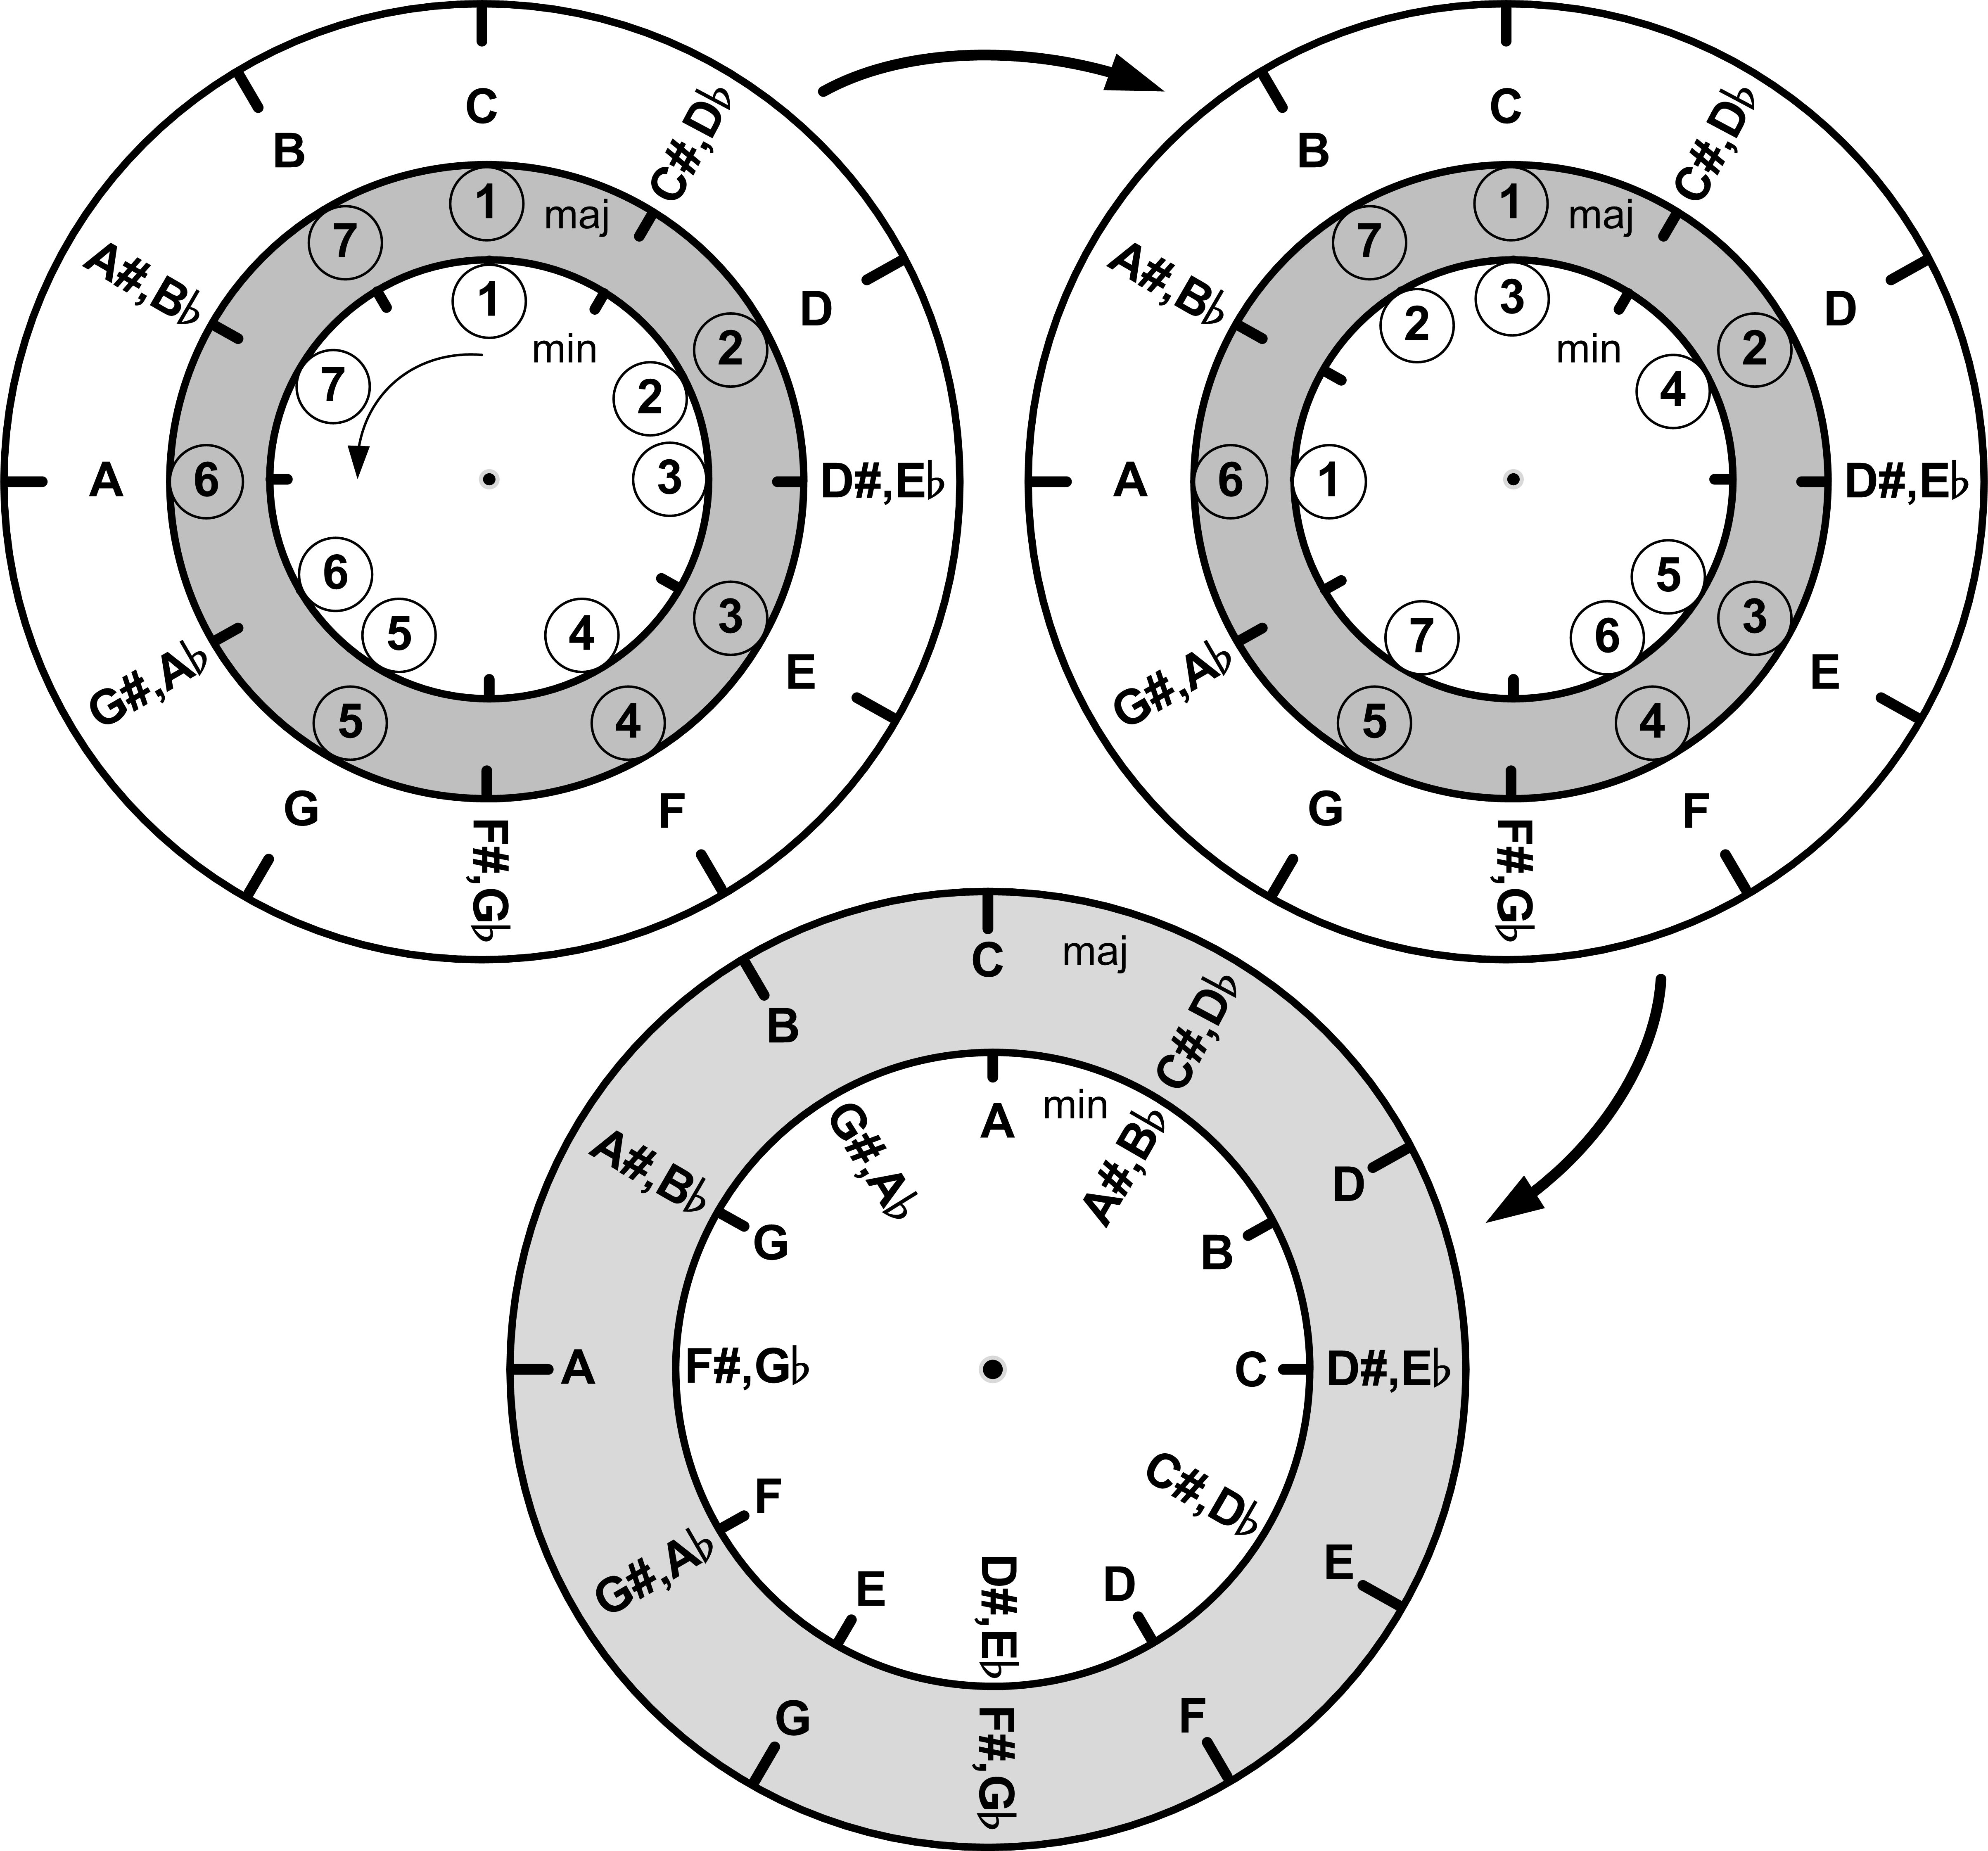
\includegraphics[scale=0.5]{fig/kvinto-kvarto/minor-major-mapping} 
    \caption{Соответствие тоник параллельных мажорных и минорных тональностей}\label{fig:harmony:kvinto-kvarto:minor-major-mapping}
\end{figure}

Если на получившемся приборе совместить шестую ступень мажорного лада с первой ступенью минорного лада (ну или первую ступень мажора с третьей ступенью минора), то будет видно, что они имеют сходную интервальную структуру и порождают параллельные тональности, т.е. тональности, в которые входят одинаковые ноты. Зафиксируем в таком положении кружки со ступенями и будем проворачивать круг с нотами. На рисунке \ref{fig:harmony:kvinto-kvarto:minor-major-mapping} показана ситуация, когда первая ступень мажора указывает на тонику ДО(C), а первая ступень минора --- на тонику ЛЯ(A). ДО-мажор и ЛЯ-минор --- параллельные тональности. Видно, что на внешнем кругу с нотами, тоника параллельной минорной тональности находится на расстоянии трех секторов против часовой стрелки от соответствующей тоники мажорной тональности. Полное соответствие тоник параллельных мажорных и минорных тональностей представлено на рисунке \ref{fig:harmony:kvinto-kvarto:minor-major-mapping}.

Вернемся к нашей <<квинто-квартовой>> перестановке нот и выпишем для неё (во внутренней части круга) тоники параллельных минорных тональностей. Получим предварительный вариант круга, представленный на рисунке \ref{fig:harmony:kvinto-kvarto:kvinto-kvarto-parallel}.

\begin{figure}[!ht]
    \centering
    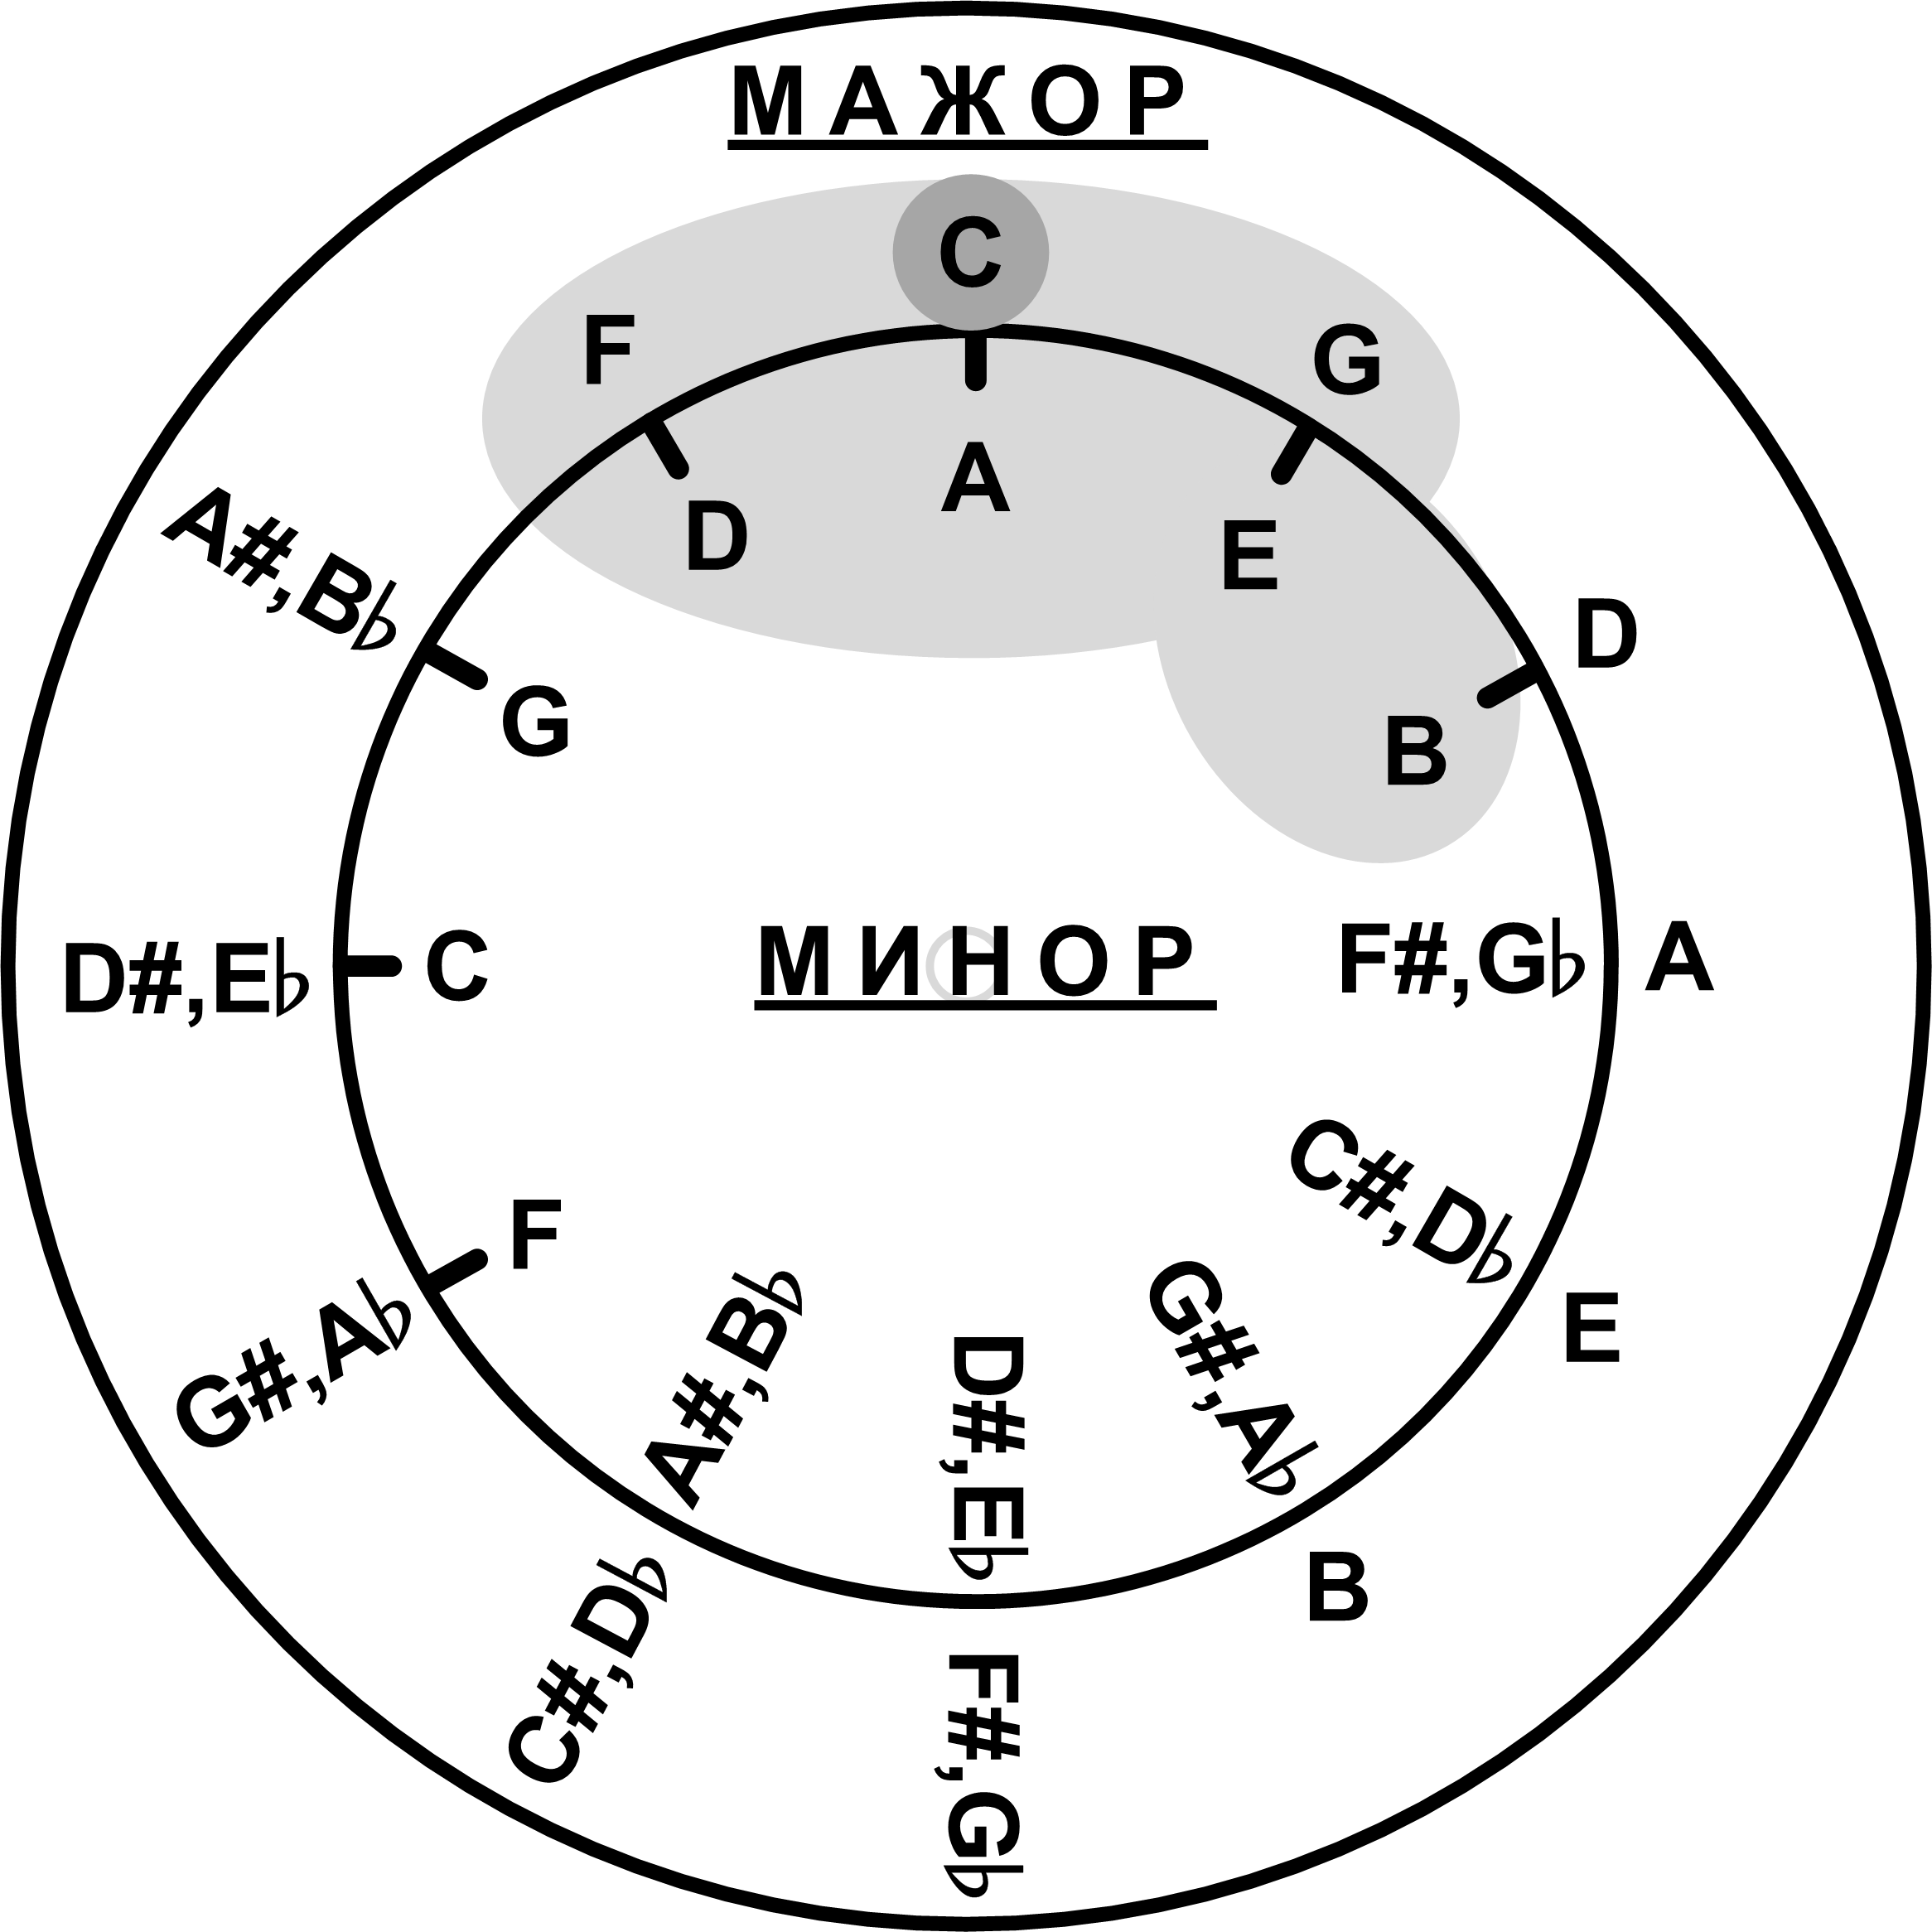
\includegraphics[scale=0.5]{fig/kvinto-kvarto/kvinto-kvarto-parallel} 
    \caption{Квинто-квартовый круг параллельных минорных и мажорных тональностей (базовая версия)}\label{fig:harmony:kvinto-kvarto:kvinto-kvarto-parallel}
\end{figure}

Если приглядеться к рисунку \ref{fig:harmony:kvinto-kvarto:kvinto-kvarto-parallel} внимательнее, то можно увидеть, что и в этом случае тоника параллельной минорной тональности находится в трех секторах. TODO
